\chapter{Theoretical Framework}\label{lit}

\section{Spatial politics and everyday life}

\dcap{I}{n order to} understand the mechanism of protest and other political expressions, it is fundamental to understand the role of space. The term \textit{protest} could be understood as ``any action, act, or statement expressing (emphatic) objection to or dissent from something'' \citep{_protest_2007}. Space, either physical or metaphorical, is where these action, act, or statement take place. The concept of space has became an important component in contemporary literatures and theories of politics and geography.\ %
\marginnote{{``(Social) space is a (social) product. [\ldots] that in addition to being a means of production it is also a means of control, and hence of domination, of power;''} \\\noindent\citep[p.~26]{lefebvre_production_1991}}%
Urban space is understood as not only a physically defined area, but a complicated mix of, as defined by Lefebvre, perceived, conceived, and lived space \citep{schmidt_henry_2008}. Being \textit{in} a city, apart from being inside its geographical border, also means conceiving and picturing the city and the image of the city, and experiencing the everyday life practiced by all residents in the city. The new image and experience thus produced are also fed back to and become part of the city. Space is where human activities take place, while it is also being constantly produced and reproduced by these activities; it creates the political relation between individuals, which brings them together but meanwhile disclose the distinctions between them (\citealp{canovan_politics_1985}, p.~634, cited in \citealp{dikec_space_2012}, p.~672). It has been argued that space is a subject or means of political control, domination, and expression of power. Instead existing as itself, space is contested, and produced by the dynamic of relations. Therefore, it could be argued that space is not political \textit{per se}, but is the ground and medium of political practice, that challenge and reproduce the established order of space through constant contestation \citep{dikec_space_2012,hou_not_2010,henaff_public_2001}.

Politics%
\marginnote{politics, \textit{n}.\\\noindent 2. The theory or practice of government or administration. \citep{_politics_2006}}%
, from its far origin in ancient Greek τὰ πολιτικά (public matters, civic affairs), has been tightly related to the concept of city, from the ancient Greek city-state i.e.\ \textit{polis} (πόλις) to a modern city. \citet[p.~93]{arendt_introduction_2005} argues that politics ``deals with the coexistence and association of \textit{different} men'', that is the fundamental of communal life. Living in a city means an individual obtains freedom by being with others who are marked as equal to them, therefore. The spatial existence of the city not only define the land but also the place where this political freedom is guaranteed. \citeauthor{ranciere_et_2009} (\citeyear{ranciere_et_2009}, cited in \citealt[p.~673]{dikec_space_2012}) argues that politics reconfigures the orders of time and space, hierarchies of places, therefore institutionalised and legitimised forms of domination, which instituted by the form of symbolisation he defined as \textit{police}. Politics in this sense is related to the distribution of space: the function of the space, the right to access the space, etc. Through opening the space, politics then challenges the established order and make new distributions and relations \citep{ranciere_politics_2003}. In terms of governance, which referring to the relations between governor (now usually means the government, or the state) and governed, the central question turns into the process of decision-making: how these decisions are made, what actors are (and are empowered to be) involved in the process, and in whose interest \citep{martin_space_2003}. A more participatory process would allow citizens to be ``deliberately included in the future'' \citep[pp.~216]{arnstein_ladder_1969}, yet this process is also constantly under contestation, as those in power resist to the redistribution of power \citep{arnstein_ladder_1969}. In short, the symbolisation of police institute the order of time and space based on the power relationship between the governed and the governor in the city, this practice of governance then become politics. Space, especially so called public space, which is the medium and ground of the politics, is the arena of political activities that either challenge or maintain the established order.

Public space has long been an important component of cities all over the world but hard to accurately defined. In Burmese,\marginnote{
\includegraphics[width=2in]{mmpublic.pdf}\\\noindent``Gathering space'' in Burmese.} there is no has same meaning as what ``public space'' means in Englishg, so the phrase has to be translated to "gathering space". In Chinese,\marginnote{\vskip4mm\noindent{\LARGE 公共空间}\\\vskip2mm\noindent``Public space'' in Chinese.} the word "public" is frequently been understood as ``owned by the state (or an organisation)''. However, what in common is, public spaces are not private, they are not owned by a single individual. In most cities there are places that accessible by the public, in which people are able to gather, socialize, run business, or sometimes protest. These spaces can be square, market, street, park, etc. \citet[p.~35]{henaff_public_2001} define public space as ``simultaneously: open to all, well known by all, and acknowledged by all\ldots\ it stands in opposition to private space of special interests''. Planning as a kind of act, embodies the interntion that power holders tend to shape the planned subject i.e.\ urban space based on their interest. However, public spaces provide the ground for people, citizens, have-nots, to loosen the given order of space and produce opportunities to new ``perceptions, attitudes, and behaviors'' \citep[p.~14]{franck_tying_2006} by challenging or disrupting the intended use of these space, take the space out of the context that has assigned features and nothing unpredictable would happen. These unintended use could be legitimised or not legitimised, impromptu or scheduled, temporary or permanent \citep{franck_tying_2006}. \citet{hou_not_2010} defines the public space that oppose the solely control, regulate, and maintain of state as ``insurgent public space'', the public space can be turned into the ground against the regulation and privatization. According to Maurice Blanchot \citep[cited in][]{sheringham_indeterminacy_2006}, the everyday\footnote{Originally referred as the \textit{quotidien}.} inherently eludes definition, that ``a sector most at the mercy of legislation and bureaucracy was at the same time refractory to such limitation'' \citep[p.~18]{sheringham_indeterminacy_2006}. The everyday life is ``potentially the present, alive with the force of lived but uncategorizable experience'' \citep[p.~17]{sheringham_indeterminacy_2006}. Therefore, it could be argue that the potential that embedded in the practice of everyday life that challenging the order, which established or planned by the power holder. And this process, intended or unintended, by which the power holder is challenged, could be political.


The practice that challenges the established order could occur in varies forms, in fact, it is inexhaustible, something would always remains uncertain, and through which the possibilities of everyday life are maintained \citep{lefebvre_critique_1991}. The massive activity of ``square dancing'' in China is an interesting example\marginnote{``{[O]ne Beijing {\rm yangge} dancer pointed out that ``good health and friends are the most important things in life,'' and that their group dancing is a basic ``{\rm human right}'' that belongs to both natives and visitors of any age in Beijing.''}\\\noindent(\citealp{brownell_training_1995}, cited in \citealp[p.~33]{chen_dancing_2010})}. In cities all over China, peoples, mostly middle-aged or old, gather and dance in the public, with loud, energetic music playing. The group size varies from four to five people to huge groups with more than one hundred people. These groups improvised any available space as the site for dancing, from ordinary public spaces such as squares and parks to road side, building entrances, and parking lots (see figure \vref{fig:squaredance}). This activity became an important element of dancers' life, providing major socializing and maintenance of health for many, with some elder people even use it as a therapy. To support their own practice, their appropriating of the public space ``unintentionally but effectively developing new typologies of hybrid use'' (\citealp{de_certeau_practice_1984}, \citealp[cited in][p.~22]{chen_dancing_2010}) for the spaces designed by urban planners. The square dancing has also been complained a lot, in a few cases, even violent attacked \citep{jacobs_cutting_2015} by residents, usually for making noise and occupying space. In June 2017 during gaokao\footnote{Gaokao is the Chinese annual National Higher Education Entrance Examination, this exam is a prerequisite for all normal student in China mainland to take the undergraduate level education.}, groups of dances in Hunan province collectively decided to stop dance for 10 days, to create a quiet environment for students to prepare for the exam \citep{xinying_squares_2017}. The dancing groups sometimes are evicted for these complains, sometimes migrate to other spaces as compromise, but always searching spaces in the city to be ``loosened'', ``tailoring a city to fit the contours of their everyday lives'' \citep{chen_dancing_2010}.

\begin{figure}[!htbp]
	\centering
	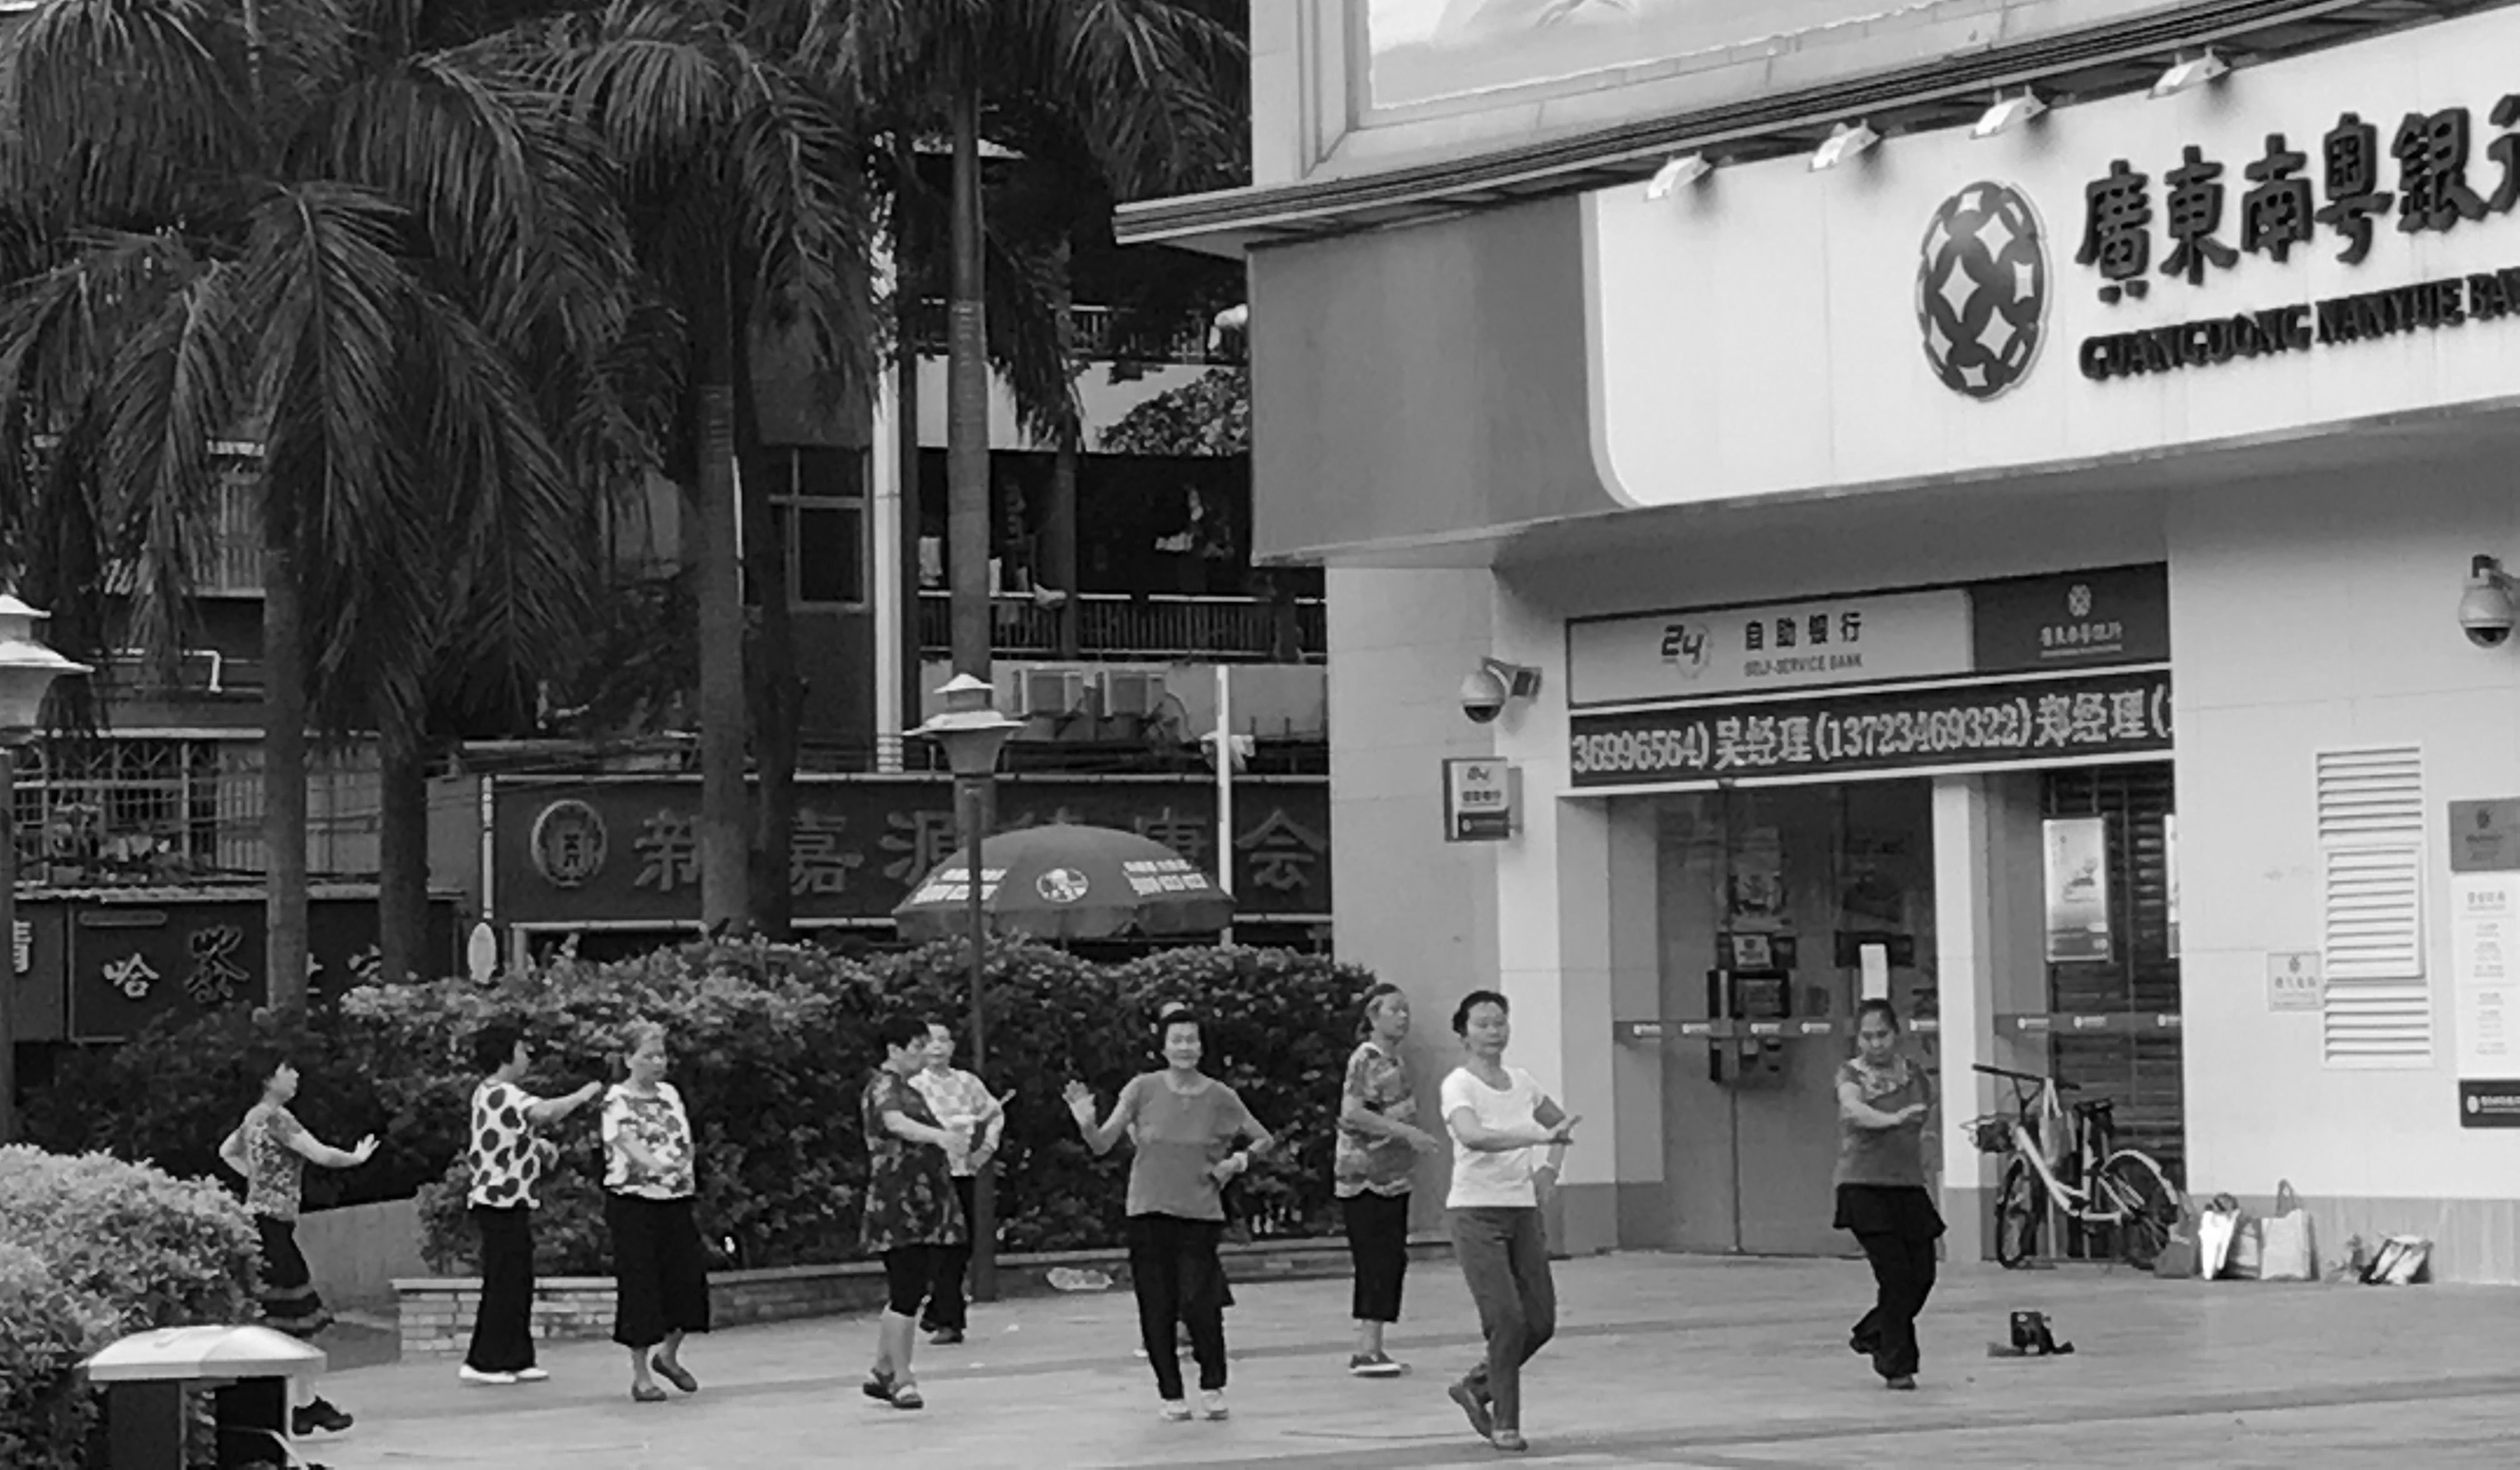
\includegraphics[width=\textwidth]{squaredance.jpg}
	\caption[A group of square dancer dancing in an open space in front of the gate of a bank]{A group of square dancer dancing in an open space in front of the gate of a bank in Shenzhen, Guangdong China.}
	\label{fig:squaredance}
\end{figure}

The everyday practice can also become a form of resistance. Scott argues that especially for the subordinate classes (this term is referred to those alienated due to lack of economic ability, political power, and social capital), it is nearly the only way of resist, since they have ``rarely been afforded the luxury of open, organized, political activity'' \citep[p.~xv]{scott_weapons_2008}. Through his research in Malaysian village Sedaka\footnote{It is not the real name of the village but an alias given by the author, as he claimed.}, the class contradiction was created by the change of the production structure. The introduction of the double-cropping and mechanization from the state gives large landowners in the village opportunity to decrease their dependency of hiring harvest workers. Therefore the traditional economical balance within the village, as it is somehow a closed agricultural economic system, that poorer people can gain \textit{zakat peribadi}\footnote{A kind of ``private Islamic tithe''. \begingroup\mancite\citep[p.~121]{scott_weapons_2008}\endgroup} from doing harvesting work for landowners as a kind of gift, but which is widely accepted as a convention that became part of the anticipated wage, is disrupted. To resist this new order, the subordinate class then protest through the practice of everyday activity. For example, the villagers uses the village gate, which was originally used for charging the passing by vehicles, in order to cover the cost maintaining the path, to stop the paddy dealers' trucks. While the trucks stopping, villagers then haul ganny sacks of paddy from it. \marginnote{{``This method of passive resistance, provided it was not expressed as open defiance, was nearly unbeatable, it reinforced the Haviks' stereotype concerning the character of low caste persons, but gave them little recourse to action.''}\\\noindent\citep{silverberg_social_1968}}This is however connived by the large farmers, and became a subsidization paying to the subordinate neighbors, as the land owners reduce the benefit of workers, the social domination power constructed through this relationship is also reduced, then to maintain the stability of tenancy and reliable labour force. This resistance that practiced to recreate the balance, requires little coordination, planning, and knowledge; it ``make use of implicit understandings and informal networks''; and does not have any direct conflict with authorities. \citet[p.~xvi]{scott_weapons_2008} defined this as the ``everyday forms of peasant resistance'' and ``ordinary weapons of relatively powerless groups''.

\section{Virtual space: another dimension of city}

The ongoing discussion and literatures of social space in the field of urban design is flourishing, however, most researchers consider the physical space of city as the medium of the social space. The integrity\ \marginnote{{``\sc everybody should understand computers}.\\\noindent{[\ldots]}\\\noindent {Computers are simply a necessary and enjoyable part of life, like food and books. Computers are not everything, they are just an {\rm aspect} of everything, and not to know this is computer illiteracy, a silly and dangerous ignorance.''}\\\noindent\citep[p.~2]{nelson_computer_1974}}and unpredictability of time and space brought by the ``electric age'' have not been paid much attention to \citep[p.~4]{mcluhan_introduction_1994}. In the 21st century, along with the rapid development of information technology, mobile device, and social network, the Internet became an increasingly important part of people's life, it massively changed the way people receive and process information, communicate, consume, and experience the world. \textit{Virtual space} here represent the extended part of social space by the new media; it does not physically exist---it never added (or removed) anything on the world map; it is built by all kinds of information that stored in mediums created by human, from book to flash disk, and being active by communication, from eye contact on the street to text messages on mobile phones. As keyboards and microphones are actually extension of hands and mouths that delivers language, screens are extension of eyes, the virtual space of Internet, culture, and language therefore extends and accelerates the spatial constructed space that we are living in, ``affects, the whole psychic and social complex'' \citep[p.~4]{mcluhan_introduction_1994}. It could therefore be argued that the social relationship, power structure, and political practice, would also have their extension and reflection in the virtual space. Due to the properties of the virtual space, these relationships, structures, and practices in the virtual space could have similarities and distinctions with those take place in the physical space.
\begin{marginfigure}
	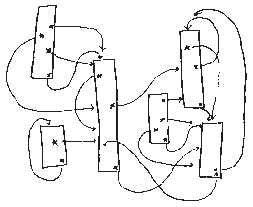
\includegraphics[width=\textwidth]{hypertext.pdf}
	\caption[A Hypertext system]{A hypertext system, from \citeauthor{nelson_computer_1974} (\citeyear{nelson_computer_1974}, p.~\smallcaps{dm47}).}
	\label{fig:hypertext}
\end{marginfigure}

In past decades, the many new properties of \ict s have been recognized and made use of, thus generated new form of culture, new life style, and ``new way of doing politics'' \citep[p.~198]{juris_new_2005}. In his research of anti-corporate globalization activists, \citeauthor{juris_new_2005} found that facilitated by several features of Internet, such as long-distance coordination, horizontal collaboration, highly flexible and decentralized network forms, activists developed their new, and more efficient way of practice, they can reach thousands of activists immediately and easily collaborate between different countries. It has been argued that the Internet and \ict s has faded the borders of time and distance \citep{juris_new_2005,harlow_collective_2012}, that information on the internet could be accessed by all the user almost equally: ``the geographical proximity and content availability are independent of each other'', information could be copied almost immediately and freely \citep[p.~179]{boyle_foucault_1997}, old information is equally easy to access as new ones, neither be worn or damaged through time. The emergence of technologies, especially \ict s, revolutionarily accelerated the process of globalization while the decentralized structure of the Internet removed the local dependency on other methods of exchanging information, thereby creating an alternative global discourse and understanding \citep{chadwick_internet_2006,dencik_alternative_2013}. \marginnote{``We now have the capacity to find common ground with people we will never meet but who we will meet through the Iinternet and through all the modern means of communication[\ldots]''\\\noindent(\citealp{brown_wiring_2009}, \citealp[cited in][p.~1219]{dencik_alternative_2013})} \citet[p.~205]{juris_new_2005} also notes that the virtual space ``can be incorporated into more everyday forms of social, economic, and political life''. Activists in Barcelona use Internet-based collaborative software to ``collectively produce documents regarding real-world initiatives'', they achieved the project smoothly in the intertwined virtual and physical space. It could be argued that the virtual space here is complementary to physical space, and through which the same purpose and practice could be conducted as in the physical space.

However,\marginnote{``[L]aw is a command backed by threats, issued by a sovereign who acknowledges no superior, directed to a geographically defined population which renders that sovereign habitual obedience.''\\\noindent(\citealp{austin_province_1954}, cited in \citealp{boyle_foucault_1997})} it should be noted that the Internet did not become a utopia. \citet{curran_why_2012} argues that the central weakness of the theorising around the Internet is that they mostly focused on the technology while the limits of social context is neglected. Many fantasies created by the advantage of \ict s including Internet technologies such as synchronicity and overcoming the physical distance is only based on the fact that the technology itself is fully accessible, in fact the availability of technology is tightly bound to the political and economical environment of users, which highly depends on actual location of the users. The Internet did bring new possibilities of communication, but only for those places that could afford its infrastructure and willing to embrace it. There is still a huge portion of population with no access to the Internet (see figure \vref{fig:internetpopulation}), while some countries ban or restrict the access to the Internet, such as the Great Firewall of China i.e.\ the \gfw. \citeauthor{curran_misunderstanding_2012} (\citeyear{curran_misunderstanding_2012}, cited in \citealp{dencik_alternative_2013}) lists several limitations of Internet regarding the discourse of globalization, including:%
\begin{figure*}[!htbp]
	\centering
	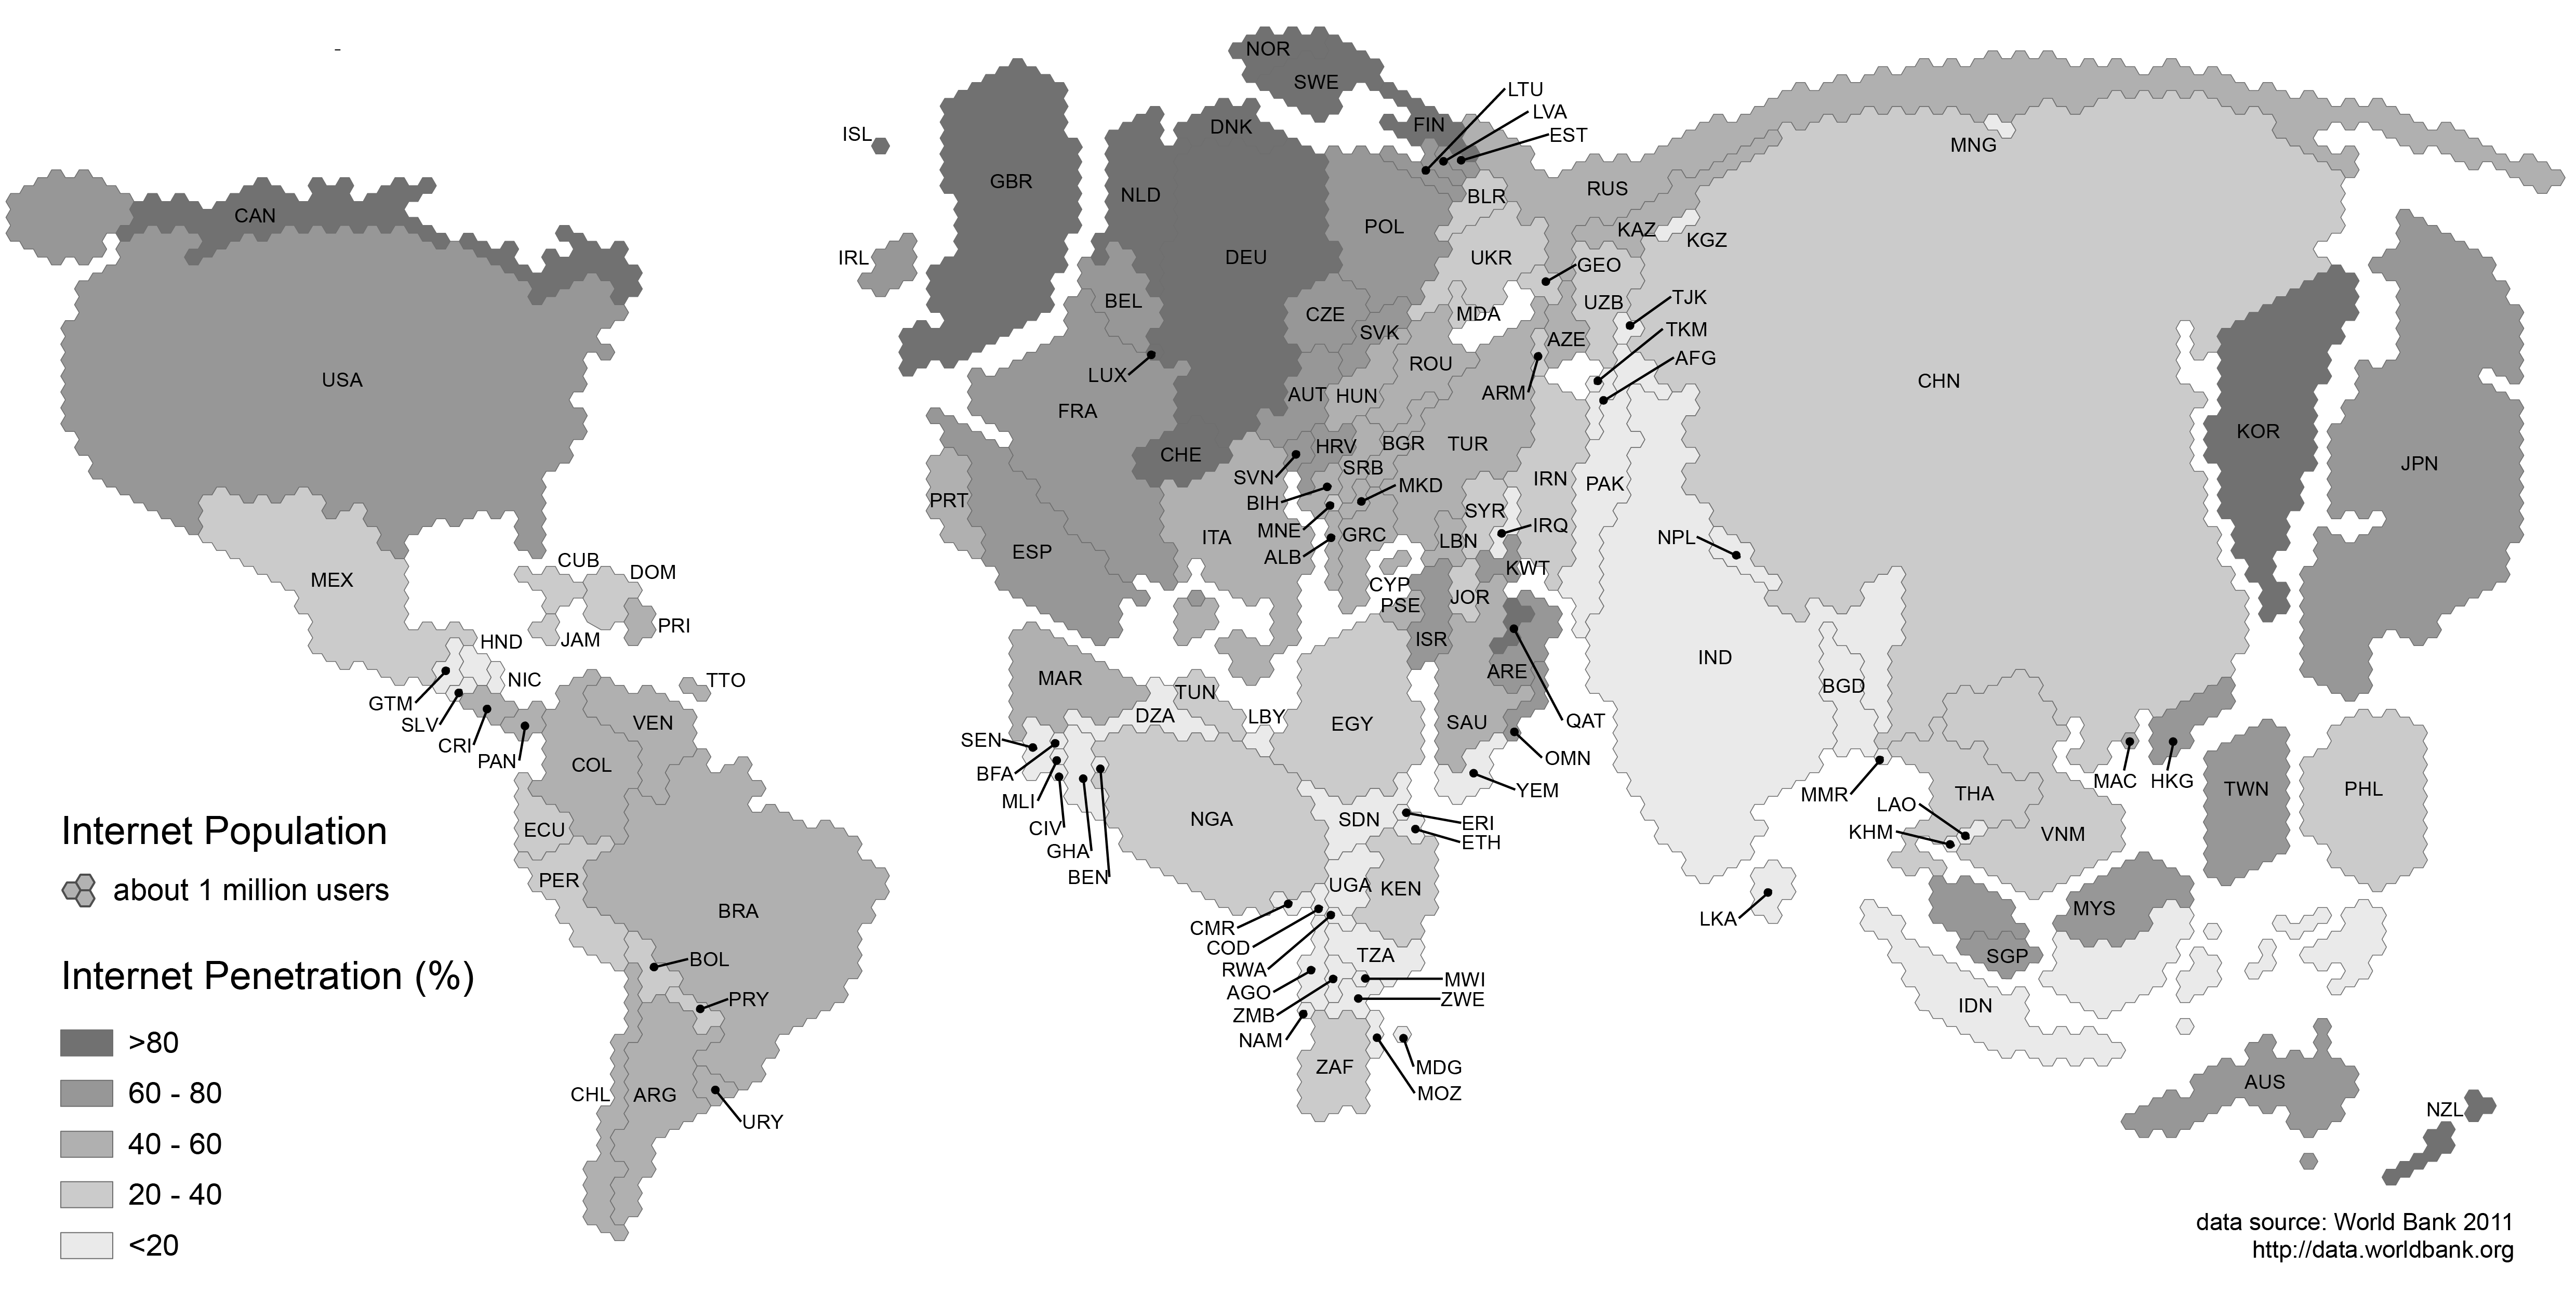
\includegraphics[width=\textwidth]{InternetPopulation.png}
	\caption[Internet population and penetration based on 2011 data]{Internet population and penetration based on 2011 data, this map illustrates the total number of Internet users in a country as well as the percentage of the population that has Internet access, from \citet{graham_internet_2013}.}
	\label{fig:internetpopulation}
\end{figure*}
\begin{enumerate}
	\item the world is very unequal and this limits participation in an internet-mediated global dialogue;
	\item the world is divided by language and only 15\% of the population understands English;
	\item language is a medium of power so those writing or speaking in English will reach a much larger public than those conversing in, say, Arabic;
	\item the world is divided by bitter conflicts of value, belief and interest;
	\item nationalist cultures are strongly embedded in most societies;
	\item authoritarian governments have developed ways of managing the net and of intimidating would-be critics;
	\item inequalities within countries – not just between them – can distort online dialogue.
\end{enumerate}
The differences in language, culture, and value actually become the border and distance in the virtual space. In the research conducted by \citet{dencik_alternative_2013}, the author detailed the efforts of website OhmyNews, the very successful citizen reporter platform expanded itself to the global scale in 2004, opening its English version OhmyNews International. According to the founder \citet{oh_end_2004},```Every Citizen is a Reporter' has been applied only to Korean speakers. Now it will grow to include people everywhere''. However, the attempt failed, OhmyNews International stopped its citizen journalism feature in 2010, due to limits of funding and difficulties of handling stories from worldwide. It is pointed out that in 2009--2010 in content produced in the site, Europe and North America took the largest share, and only 4\% of which is about Africa. The principle of ``Every citizen is a reporter'' actually resulted in those those who were from most powerful countries, who have better access to the Internet, better English skill, would have most voice, even on the Internet. \citet{dencik_media_2011} argues that the transformative potential in the virtual space as political space, rather than necessarily challenging the dominant power structure, could actually replicating it, or even legitimizing it.

\section{Summary}

To summarize, this chapter explored the idea of conversion between everyday and political expressions, and the relation between physical and virtual spaces. As the term \textit{politics} could be defined as the activities that challenge or maintain the established order, when lacking power or resources for direct defiance to the power holders, the political expression of subordinate classes would transform from explicit action or discourse to implicit ones. Through the creative use of public space, which has been usually designed with clear purpose, the practice of everyday life from subordinate people could blurs the discipline created by the authorities, and create contested insurgence space that claims their own demand.

Based on Mcluhan's theory of medium as extension of human, this chapter also reviewed the idea that the virtual space i.e.\ the metaphorical space created by \ict s as an extension of the physical urban space. On one hand, the nature of the virtual space can break certain borders in the physical space, and thus accelerate or even initiate new social communication and activity; on the other hand, due to the complex reality of imbalanced distribution of Internet infrastructure, language, and other social economical factors, the power relations and politics appear in the physical world have often been extended into the virtual space, that the virtual space sometimes does not fix the power difference, but continues it, or even amplifies it.

\begin{figure}[!htbp]
	\centering
	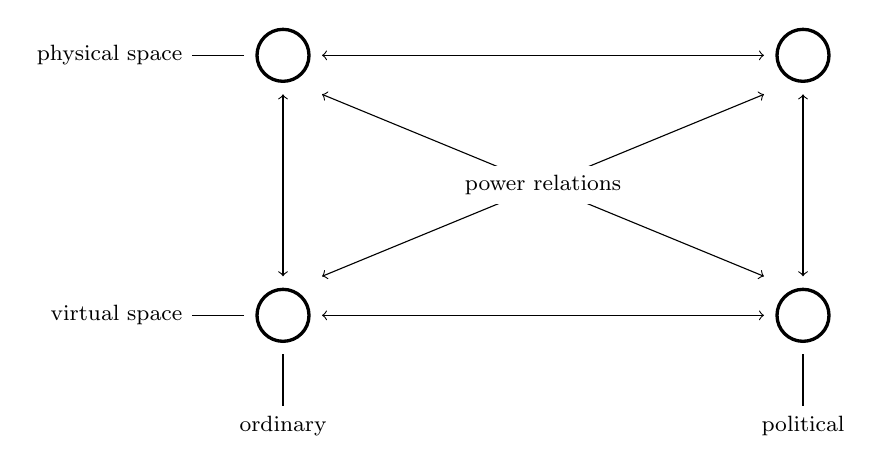
\begin{tikzpicture}[x=1.3in, y=1.3in, font=\footnotesize]
	\draw[very thick] (1,1) circle [radius=.1];
    \draw[very thick] (1,2) circle [radius=.1];
    \draw[very thick] (3,1) circle [radius=.1];
    \draw[very thick] (3,2) circle [radius=.1];

    \draw [<->] (1,1.15) -- (1,1.85);
    \draw [<->] (3,1.15) -- (3,1.85);
    \draw [<->] (1.15,2) -- (2.85,2);
    \draw [<->] (1.15,1) -- (2.85,1);

    \draw (1,0.85) -- (1,0.65) node [below] {ordinary};
    \draw (3,0.85) -- (3,0.65) node [below] {political};
    \draw (0.85,1) -- (0.65,1) node [left] {virtual space};
    \draw (0.85,2) -- (0.65,2) node [left] {physical space};

    \draw [<->] (1.15,1.15) -- (2.85,1.85);
    \draw [<->] (1.15,1.85) -- (2.85,1.15);

    \node [rectangle, fill=white] at (2, 1.5) {power relations};
\end{tikzpicture}


	\caption[A summary of the theoretical framework]{A summary of the theoretical framework.}
	\label{fig:theo}
\end{figure}
